\documentclass[11pt]{article}

\usepackage[a4paper,margin=1in]{geometry}
\usepackage[T1]{fontenc}
\usepackage[utf8]{inputenc}
\usepackage{lmodern}
\usepackage{microtype}
\usepackage{amsmath,amssymb,amsthm,mathtools}
\usepackage{booktabs}
\usepackage{graphicx}
\usepackage{enumitem}
\usepackage[numbers,sort&compress]{natbib}
\usepackage{xcolor}
\usepackage{xurl}
\usepackage[colorlinks=true,linkcolor=blue!55!black,citecolor=blue!55!black,urlcolor=blue!55!black]{hyperref}
\usepackage[nameinlink,noabbrev]{cleveref}

\setlength{\parindent}{1.4em}
\setlength{\parskip}{0.15em}
\setlist{itemsep=0.25em,topsep=0.35em}

\newtheorem{theorem}{Theorem}[section]
\newtheorem{proposition}[theorem]{Proposition}
\newtheorem{lemma}[theorem]{Lemma}
\newtheorem{corollary}[theorem]{Corollary}
\theoremstyle{definition}
\newtheorem{definition}[theorem]{Definition}
\theoremstyle{remark}
\newtheorem{remark}[theorem]{Remark}

\newcommand{\R}{\mathbb R}
\newcommand{\C}{\mathbb C}
\newcommand{\E}{\mathbb E}
\newcommand{\uc}{u_{\mathrm c}}
\newcommand{\cK}{\mathcal K}
\newcommand{\cA}{\mathcal A}
\newcommand{\Id}{\operatorname{Id}}
\newcommand{\diag}{\operatorname{diag}}
\newcommand{\spec}{\operatorname{spec}}
\newcommand{\Arg}{\operatorname{Arg}}
\newcommand{\norm}[1]{\left\lVert #1\right\rVert}
\newcommand{\one}{\mathbf 1}

\title{\textbf{Continuum Spectral Convergence and}\\
\textbf{Time--Resolution Windows for Gaussian}\\
\textbf{Quadratic Markov Operators}\\
\large Collectively Compact Nystr\"om Limits and Topology-Dependent Sampling}
\author{Liang Wang\\
\small School of Artificial Intelligence and Automation,\\[-0.2em]
\small Huazhong University of Science and Technology, Wuhan 430074, P.R. China\\
\small \texttt{wangliang.f@gmail.com}}
\date{July 2026}

\begin{document}

\maketitle

\begin{abstract}
Finite Gaussian transition matrices for logarithmically driven quadratic maps
have an exact parameter-response calculus, but a fixed-dimensional theorem
does not by itself justify simultaneous growth of observation time and spatial
resolution.  We construct the corresponding fixed-noise continuum operator
and derive sharp distinctions among deterministic probability propagation,
weak observable estimation, and strong matrix estimation.

For $f_u(x)=1-u x^2$ on $[-1,1]$ with fixed Gaussian width $\sigma>0$, the
normalized kernel defines a compact, strongly positive, operator-norm analytic
Markov family $\cK_{\sigma,u}$ on $C([-1,1])$.  Its Perron eigenvalue is simple,
and all other spectral values lie strictly inside the unit disk.  The midpoint
Nystr\"om operators converge strongly and collectively compactly, together
with their first two parameter derivatives.  Hence every nonzero isolated
resonance is spectrally exact.  For a simple resonance, its eigenvalue,
right Nystr\"om eigenfunction, and parameter and eigenphase derivatives converge at
order $h^2$, where $h=2/d$.

Let the response scale be $s_T=(\log T)^{-p}$.  A deterministic resonance
response survives the joint limit if $h^2=o(s_T)$.  For row-normalized expected
flow, the same result holds uniformly after one Gaussian smoothing step; if an
atomic initial row is retained, the additional initial-layer condition is
$d/T=o(s_T)$.  Sampling introduces topology-dependent upper restrictions.
With $N_i\asymp T/d$ transitions per source row, one smooth observable has
error $O_{\mathbb P}(\sqrt{d/T})$, whereas an entire empirical row in total
variation has mean error $O(d/\sqrt T)$.  Thus the leading dimension windows
are
\[
  (\log T)^{p/2}\ll d(T)\ll\frac{T}{(\log T)^{2p}}
  \quad\text{for one weak observable},
\]
and
\[
  (\log T)^{p/2}\ll d(T)\ll\frac{\sqrt T}{(\log T)^p}
  \quad\text{for strong matrix control}.
\]
Only the latter directly provides topology-robust perturbation control for a
nonnormal spectrum.

Numerically, fixed-width resonance and eigenphase-response errors follow
$d^{-2}$ through $d=50{,}000$.  Independent row-sampling experiments recover
dimension exponents $1.0046$ for total variation and $0.4827$ for a smooth
observable, in agreement with the theory.  The results neither identify a
Markov resonance with a Riemann zero nor construct a self-adjoint spectral
realization.
\end{abstract}

\noindent\textbf{Keywords:} compact Markov operator; Nystr\"om method;
collectively compact approximation; nonnormal resonance; double limit;
multinomial sampling; quadratic map.

\medskip
\noindent\textbf{MSC 2020:} 47A58; 45C05; 65R20; 37H20; 60J10.

\section{Introduction}

Finite transition matrices are useful numerical models only after their
resolution limit is specified.  This is particularly important for
nonnormal Markov matrices: entrywise convergence, a visually stable phase
plot, and convergence on one observable are weaker than operator control of
the spectrum.

The prime-dynamics program began with a deterministic-chaos model of sieve
words \citep{Wang2026Published} and subsequently separated exact symbolic,
Fourier, and parity statements from conjectural spectral interpretations
\citep{WangParity2026}.  A related numerical manuscript constructs
Gaussian-smoothed transition matrices for a logarithmically driven quadratic
map and compares selected eigenphases with zero ordinates
\citep{WangSpectralFlow2026}.  A theoretical audit showed that raw phase fits
can be driven by symmetry and smooth counting laws and proved fixed-resolution
operator freezing \citep{WangObstructions2026}.

The next layer derived exact first and second derivatives of the finite
Gaussian matrix, proved a twice-the-tail truncation identity, and resolved the
difference between an unweighted matrix average and row-normalized accumulated
flow \citep{WangGaussianResponse2026}.  At fixed dimension, every
positive-density row weighting preserves the leading unanchored response
\[
  (\log T)^p(Q_T-K_d(\uc))\longrightarrow\kappa K_d'(\uc).
\]
Sparse computations through dimension $50{,}000$ exhibited second-order grid
convergence of one nonreal resonance and its phase derivative.

Two questions remain.  First, does the matrix spectrum converge to the
spectrum of a specified continuum operator, without spectral pollution?
Second, how fast may $d=d(T)$ grow while a logarithmic response remains larger
than discretization and estimation errors?

The answer to the second question depends on what is estimated.  Propagating
the complete probability vector is deterministic and has no Monte Carlo
error.  Estimating one conditional expectation from a trajectory uses about
$T/d$ visits to a source bin and therefore fluctuates at scale
$\sqrt{d/T}$.  Estimating its entire destination distribution is harder:
there are order $d$ resolved destination cells at fixed physical noise width,
and the row total-variation error is order $d/\sqrt T$.  The two errors lead
to different admissible windows.

\subsection*{Main results}

\begin{enumerate}[label=\textbf{R\arabic*.},leftmargin=3.2em]
  \item The fixed-width continuum Gaussian kernel defines a compact,
  strongly positive, analytic Markov family on $C([-1,1])$.  The eigenvalue
  $1$ is simple and is the only peripheral spectral value.

  \item Midpoint Nystr\"om operators and their first two parameter derivatives
  converge strongly and collectively compactly.  Nonzero isolated spectral
  clusters have the correct algebraic multiplicity and no spurious nonzero
  limit.

  \item A simple resonance, its right Nystr\"om eigenfunction, and its
  parameter and eigenphase responses converge at order $d^{-2}$.

  \item The deterministic logarithmic resonance response has a joint limit
  whenever $d^{-2}=o((\log T)^{-p})$.  Full expected-flow normalization has
  the same limit after Gaussian smoothing; an included atomic initial layer
  contributes the additional bias $O(d/T)$.

  \item Conditional estimation of a single bounded observable has
  root-mean-square error $O(\sqrt{d/T})$.  Estimation of a complete row in
  $\ell^1$ has mean error $O(d/\sqrt T)$, and this order persists for the
  maximum of independently stratified rows.

  \item Combining bias and variance gives distinct weak-observable and
  strong-matrix windows.  The strong window is the appropriate sufficient
  condition for black-box perturbation of a nonnormal spectrum.
\end{enumerate}

\subsection*{Scope}

The continuum object in this paper is a compact Markov operator at fixed
physical noise width.  Its complex resonances are decay and oscillation modes,
not self-adjoint energies.  The six-sigma numerical width inherited from the
preceding paper is historically target-informed; it is used only to audit
resolution convergence and is not an arithmetic prediction.  No zeta zero is
loaded or compared in the new experiments, and no assertion about the
Riemann hypothesis is made.

\section{The fixed-noise continuum operator}
\label{sec:continuum}

Let $I=[-1,1]$, fix $\sigma>0$, and let $u$ range over a compact real interval
$J$.  Put
\begin{align}
  f_u(x)&=1-u x^2,\label{eq:quadratic}\\
  w_u(x,y)&=\exp\left(-\frac{(y-f_u(x))^2}{2\sigma^2}\right),\label{eq:weight}\\
  Z_u(x)&=\int_Iw_u(x,z)\,dz,\qquad
  q_u(x,y)=\frac{w_u(x,y)}{Z_u(x)}.\label{eq:density}
\end{align}
Define on $C(I)$
\begin{equation}\label{eq:continuum-operator}
  (\cK_u g)(x)=\int_Iq_u(x,y)g(y)\,dy.
\end{equation}
We suppress $\sigma$ when it is fixed.

\begin{theorem}[Compact analytic Markov family]\label{thm:continuum}
The family \eqref{eq:continuum-operator} has the following properties.
\begin{enumerate}[label=(\roman*),leftmargin=2.2em]
  \item $\cK_u$ is a positive contraction on $C(I)$,
  $\cK_u\one=\one$, and $\cK_u$ is compact.
  \item $\cK_u$ is strongly positive: if $g\ge0$ and $g\not\equiv0$, then
  $\cK_u g>0$ everywhere.
  \item The map $u\mapsto\cK_u$ is real analytic in operator norm on a
  neighborhood of $J$.
  \item Its spectral radius is one, the eigenvalue $1$ is algebraically
  simple, and every $\lambda\in\spec(\cK_u)\setminus\{1\}$ satisfies
  $|\lambda|<1$.
\end{enumerate}
\end{theorem}

\begin{proof}
The normalized density is continuous and positive on the compact set
$J\times I\times I$.  It integrates to one in $y$, so positivity,
contractivity, and preservation of constants follow directly.  Integral
operators with continuous kernels map the unit ball to a bounded
equicontinuous family and are compact by Arzel\`a--Ascoli
\citep{Kress2014}.

Strict positivity of $q_u$ gives strong positivity.  Since $Z_u(x)$ is
uniformly separated from zero and the Gaussian is entire in $u$, all
parameter derivatives of $q_u$ are uniformly bounded on compact
neighborhoods of $J$.  Taylor expansion under the integral proves
operator-norm analyticity.

Finally, $\cK_u\one=\one$ and $\norm{\cK_u}=1$, so the spectral radius is one.
The strong form of the Krein--Rutman theorem gives simplicity of the Perron
root and excludes every other peripheral eigenvalue
\citep{Schaefer1974}.
\end{proof}

\subsection{Continuum score derivatives}

Define the score and its row mean by
\begin{equation}\label{eq:continuum-score}
  a_u(x,y)=-\frac{x^2}{\sigma^2}\bigl(y-f_u(x)\bigr),
  \qquad
  \overline a_u(x)=\int_Iq_u(x,y)a_u(x,y)\,dy.
\end{equation}

\begin{proposition}[Exact continuum derivatives]\label{prop:continuum-derivatives}
For $g\in C(I)$,
\begin{align}
  (\cK_u'g)(x)
  &=\int_Iq_u(x,y)\bigl(a_u(x,y)-\overline a_u(x)\bigr)g(y)\,dy,
  \label{eq:continuum-first}\\
  (\cK_u''g)(x)
  &=\int_Iq_u(x,y)\left[
    \bigl(a_u(x,y)-\overline a_u(x)\bigr)^2
    -\operatorname{Var}_{q_u(x,\cdot)}(a_u(x,\cdot))
  \right]g(y)\,dy.
  \label{eq:continuum-second}
\end{align}
In particular, $\cK_u'\one=\cK_u''\one=0$.
\end{proposition}

\begin{proof}
Logarithmic differentiation of $q_u=w_u/Z_u$ gives the centered score in
\eqref{eq:continuum-first}.  The derivative
$\partial_u a_u(x,y)=-x^4/\sigma^2$ is independent of $y$, so it cancels
after centering.  A second differentiation gives
\eqref{eq:continuum-second}.  The zero identities follow by integration.
\end{proof}

Let $\lambda(u)\ne0$ be a simple isolated eigenvalue, with right eigenfunction
$r_u$ and left eigenfunctional $\ell_u$, normalized by
$\ell_u(r_u)=1$.  Analytic compact-operator perturbation theory gives
\begin{equation}\label{eq:continuum-response}
  \lambda'(u)=\ell_u(\cK_u'r_u),\qquad
  \theta'(u)=\operatorname{Im}\frac{\ell_u(\cK_u'r_u)}{\lambda(u)},
  \quad\theta=\Arg\lambda.
\end{equation}
Because $\lambda\ne0$, both $r_u=\lambda^{-1}\cK_ur_u$ and the density
representing $\ell_u$ are smooth.

\section{Collectively compact Nystr\"om approximation}
\label{sec:nystrom}

Let $h=2/d$ and
\[
  c_j=-1+\left(j-\frac12\right)h,\qquad 1\le j\le d.
\]
Define
\begin{align}
  Z_{d,u}(x)&=h\sum_{j=1}^dw_u(x,c_j),\label{eq:discrete-normalizer}\\
  (\cK_{d,u}g)(x)
  &=\frac{h\sum_{j=1}^dw_u(x,c_j)g(c_j)}{Z_{d,u}(x)}.
  \label{eq:nystrom}
\end{align}
This is a finite-rank operator on $C(I)$.  At $x=c_i$ its matrix is exactly
\begin{equation}\label{eq:matrix}
  K_{ij}^{(d)}(u)
  =\frac{w_u(c_i,c_j)}{\sum_{k=1}^dw_u(c_i,c_k)}.
\end{equation}
The nonzero spectra of $\cK_{d,u}$ and $K^{(d)}(u)$ coincide, including
algebraic multiplicity.  Evaluation at the centers maps every nonzero
finite-rank eigenfunction to a matrix eigenvector, and the Nystr\"om formula
reconstructs the eigenfunction from that vector.

\begin{lemma}[Uniform stability]\label{lem:uniform}
For $u\in J$ and all sufficiently large $d$, $Z_{d,u}$ is uniformly bounded
above and away from zero.  Moreover, for $m=0,1,2$,
\[
  \sup_{d\ge d_0}\sup_{u\in J}
  \norm{\partial_u^m\cK_{d,u}}_{C(I)\to C(I)}<\infty.
\]
\end{lemma}

\begin{proof}
The midpoint sums for $Z_u$ converge uniformly in $(u,x)$, while
$\min_{J\times I}Z_u(x)>0$.  Parameter differentiation gives finite
centered score moments, bounded uniformly because $I$ and $J$ are compact
and $\sigma$ is fixed.
\end{proof}

\begin{theorem}[Strong and collective compact convergence]
\label{thm:collective}
For $m=0,1,2$ and every fixed $g\in C(I)$,
\begin{equation}\label{eq:strong-convergence}
  \sup_{u\in J}
  \norm{\partial_u^m\cK_{d,u}g-\partial_u^m\cK_ug}_\infty
  \longrightarrow0.
\end{equation}
For each $m$, the family
\[
  \{\partial_u^m\cK_{d,u}:d\ge d_0,\ u\in J\}
\]
is collectively compact.
\end{theorem}

\begin{proof}
For fixed $g$, the numerator and denominator in \eqref{eq:nystrom}, and their
first two parameter derivatives, are uniform Riemann sums of continuous
functions on a compact set.  This proves \eqref{eq:strong-convergence}.

For $\norm{g}_\infty\le1$, differentiating \eqref{eq:nystrom} with respect to
$x$ gives a uniform Lipschitz bound because $\sigma$ is fixed and the
normalizers are separated from zero.  The same applies after one or two
parameter derivatives.  Thus the union of the images of the unit ball is
bounded and equicontinuous.  Arzel\`a--Ascoli gives collective compactness
\citep{Anselone1971,Atkinson1997}.
\end{proof}

\begin{remark}[Why operator-norm convergence is not asserted]
\label{rem:no-norm}
Midpoint evaluation cannot converge in operator norm on the whole unit ball
of $C(I)$, whose elements need not share a modulus of continuity.  Collective
compactness plus strong convergence is the correct framework: it gives
spectral exactness for nonzero isolated eigenvalues without making a false
uniform quadrature claim \citep{Anselone1971,Chatelin1983}.
\end{remark}

\begin{theorem}[Spectral exactness and second-order simple branches]
\label{thm:spectral-convergence}
Fix $u\in J$.
\begin{enumerate}[label=(\roman*),leftmargin=2.2em]
  \item If $\lambda\ne0$ is an isolated eigenvalue of $\cK_u$ of algebraic
  multiplicity $m$, then every sufficiently small isolating disk contains
  exactly $m$ eigenvalues of $\cK_{d,u}$, counted algebraically, for all
  sufficiently large $d$.  Every nonzero limit point of Nystr\"om
  eigenvalues belongs to $\spec(\cK_u)$.
  \item If $\lambda$ is simple, one can choose the Nystr\"om branch
  $\lambda_d$ and its continuous finite-rank right eigenfunction $r_d$ so that
  \begin{equation}\label{eq:second-order-spectral}
    |\lambda_d-\lambda|
    +\norm{r_d-r}_\infty
    +|\lambda_d'-\lambda'|
    =O(h^2).
  \end{equation}
  If $\lambda\ne0$, then also
  \begin{equation}\label{eq:phase-second-order}
    |\theta_d'-\theta'|=O(h^2).
  \end{equation}
\end{enumerate}
The estimates are locally uniform along a compact simple branch.
\end{theorem}

\begin{proof}
Part (i) is the collectively compact spectral approximation theorem
\citep{Anselone1971,Atkinson1967,Chatelin1983}.

For a nonzero eigenvalue, the right eigenfunction and the density of the left
eigenfunctional are smooth because they lie in the ranges of $\cK_u$ and
its adjoint.  Composite midpoint quadrature is second order on these smooth
functions.  Standard Nystr\"om eigenvalue estimates therefore give
$|\lambda_d-\lambda|+\norm{r_d-r}_\infty=O(h^2)$
\citep{Atkinson1967,Atkinson1997}.  Apply the same argument to $\cK_u'$ and
the left-right formula \eqref{eq:continuum-response}; collective spectral
projections remain uniformly bounded along an isolated simple branch.  This
gives the derivative estimate.  The phase estimate follows from
$d\Arg z=\operatorname{Im}(dz/z)$ away from zero.
\end{proof}

\begin{remark}[Hard Gaussian cutoff]\label{rem:cutoff}
\Cref{thm:spectral-convergence} concerns the full Nystr\"om sum.  If each row
is truncated and renormalized, its matrix infinity-norm error is exactly
twice the omitted mass \citep{WangGaussianResponse2026}.  A fixed six-sigma
cutoff therefore approximates a fixed truncated operator to second order,
while its difference from the full operator remains a small but nonzero tail
perturbation.  Nonnormal spectral conversion additionally depends on the
left-right condition number.
\end{remark}

\section{Deterministic time--resolution limits}
\label{sec:deterministic}

Let
\begin{equation}\label{eq:schedule}
  u_n=\uc+\delta_n,\qquad
  \delta_n=\frac{\kappa}{(\log(n+c))^p}
  +O((\log(n+c))^{-p-1}),
\end{equation}
where $c>1$ and $p>0$.  Put $s_T=(\log T)^{-p}$ and define the deterministic
Nystr\"om average
\begin{equation}\label{eq:operator-average}
  \cA_{d,T}=\frac1T\sum_{n=1}^T\cK_{d,u_n}.
\end{equation}

\begin{theorem}[Deterministic spectral double limit]
\label{thm:deterministic-double}
Let $\lambda(\uc)\ne0$ be a simple isolated eigenvalue of $\cK_{\uc}$.
Let $\lambda_{d,T}$ be the corresponding eigenvalue of \eqref{eq:operator-average}.
If
\begin{equation}\label{eq:deterministic-condition}
  d(T)\longrightarrow\infty,\qquad
  d(T)^{-2}=o(s_T),
\end{equation}
then
\begin{align}
  s_T^{-1}\bigl(\lambda_{d(T),T}-\lambda(\uc)\bigr)
  &\longrightarrow\kappa\lambda'(\uc),\label{eq:deterministic-eigen}\\
  s_T^{-1}\bigl(\Arg\lambda_{d(T),T}-\Arg\lambda(\uc)\bigr)
  &\longrightarrow\kappa\theta'(\uc).
  \label{eq:deterministic-phase}
\end{align}
\end{theorem}

\begin{proof}
\Cref{lem:uniform} and Taylor expansion give, uniformly in $d$,
\[
  \cA_{d,T}
  =\cK_{d,\uc}+\kappa s_T\cK_{d,\uc}'+o(s_T).
\]
The isolated simple branch and its condition number are uniform for large
$d$ by \cref{thm:spectral-convergence}.  Hence
\[
  \lambda_{d,T}
  =\lambda_d(\uc)+\kappa s_T\lambda_d'(\uc)+o(s_T).
\]
Now $\lambda_d(\uc)-\lambda(\uc)=O(d^{-2})=o(s_T)$ and
$\lambda_d'(\uc)\to\lambda'(\uc)$.  This proves
\eqref{eq:deterministic-eigen}; the phase formula follows similarly.
\end{proof}

For $s_T=(\log T)^{-p}$, condition \eqref{eq:deterministic-condition} is
\begin{equation}\label{eq:lower-window}
  d(T)\gg(\log T)^{p/2}.
\end{equation}
There is no sampling upper bound for the unweighted deterministic average.

\subsection{Row-normalized expected flow}

Let $\nu_{n,d}$ be a row probability vector propagated by the full matrices,
\[
  \nu_{n+1,d}=\nu_{n,d}K_d(u_n),
\]
and define
\begin{equation}\label{eq:expected-flow}
  Q_{d,T;i\bullet}
  =
  \frac{\sum_{n=1}^T\nu_{n,d;i}K_{d;i\bullet}(u_n)}
       {\sum_{n=1}^T\nu_{n,d;i}}.
\end{equation}

\begin{lemma}[Uniform cell-scale occupation]\label{lem:cell-occupation}
There are constants $0<c_0<C_0<\infty$, independent of sufficiently large
$d$, such that every full Gaussian matrix with $u\in J$ satisfies
\begin{equation}\label{eq:entry-scale}
  c_0h\le K_{ij}^{(d)}(u)\le C_0h.
\end{equation}
Consequently, after one transition,
\begin{equation}\label{eq:source-scale}
  c_0h\le\nu_{n,d;i}\le C_0h
\end{equation}
for every source row.
\end{lemma}

\begin{proof}
On the compact set $J\times I\times I$, the unnormalized Gaussian weight is
between a positive constant $m_\sigma$ and one.  Its row sum lies between
$dm_\sigma$ and $d$.  Since $d=2/h$, \eqref{eq:entry-scale} follows.
A convex combination of the entries in a destination column has the same
bounds.
\end{proof}

\begin{corollary}[Expected-flow double limit]\label{cor:expected-double}
Under the hypotheses of \cref{thm:deterministic-double}, suppose either that
the initial source already satisfies \eqref{eq:source-scale}, or that the first
transition is discarded as a smoothing layer.  Then the eigenvalue and phase
of $Q_{d(T),T}$ satisfy
\eqref{eq:deterministic-eigen}--\eqref{eq:deterministic-phase}.

If an atomic initial row is retained, the same conclusion holds under the
additional condition
\begin{equation}\label{eq:initial-layer}
  \frac{d(T)}T=o(s_T).
\end{equation}
\end{corollary}

\begin{proof}
After smoothing, all row weights are between constant multiples of $h$.
The weighted slow-variation proof from \citet{WangGaussianResponse2026} is
therefore uniform in $d$: the common factor $h$ cancels between numerator and
denominator.  Uniform parameter derivatives then give
\[
  Q_{d,T}=K_d(\uc)+\kappa s_TK_d'(\uc)+o(s_T)
\]
in matrix infinity norm.  Apply the proof of
\cref{thm:deterministic-double}.

An atomic source contributes at most one unsmoothed weight to one row.  Its
row denominator is of order $Th$, so the resulting initial-layer term is
$O((Th)^{-1})=O(d/T)$.  Condition \eqref{eq:initial-layer} makes it
$o(s_T)$.
\end{proof}

\begin{remark}[Sparse cutoff and thresholds]\label{rem:sparse-occupation}
The uniform lower bound \eqref{eq:entry-scale} uses the full Gaussian kernel.
A hard cutoff or a numerical rule that discards source masses below a
threshold introduces exact zeros and can invalidate uniform occupation.
Those modifications require a separate reachability and denominator
estimate.
\end{remark}

\section{Sampling topology and empirical windows}
\label{sec:sampling}

The deterministic flow \eqref{eq:expected-flow} propagates all probabilities;
it is not a one-trajectory transition-count estimator.  We now quantify the
additional cost of empirical estimation.

For row $i$, suppose $N_i$ destination samples
$Y_{i,1},\ldots,Y_{i,N_i}$ are independent, with possibly nonidentical
probabilities $p_{i,k}\in\R^d$.  Let
\[
  \overline p_i=\frac1{N_i}\sum_{k=1}^{N_i}p_{i,k},\qquad
  \widehat p_i=\frac1{N_i}\sum_{k=1}^{N_i}e_{Y_{i,k}}.
\]
This row-stratified model isolates conditional transition sampling.  It also
applies conditionally in settings where visits to each source row supply an
appropriate concentration inequality.

\begin{theorem}[Strong and weak row errors]\label{thm:sampling}
Assume $N_i\asymp T/d$ uniformly in $i$.
\begin{enumerate}[label=(\roman*),leftmargin=2.2em]
  \item For every row,
  \begin{equation}\label{eq:l1-mean}
    \E\norm{\widehat p_i-\overline p_i}_1
    \le\sqrt{\frac d{N_i}}
    =O\left(\frac d{\sqrt T}\right).
  \end{equation}
  If rows are sampled independently, then
  \begin{equation}\label{eq:max-row}
    \E\max_{1\le i\le d}\norm{\widehat p_i-\overline p_i}_1
    =
    O\left(
      \frac d{\sqrt T}
      +\sqrt{\frac{d\log d}{T}}
    \right)
    =O\left(\frac d{\sqrt T}\right).
  \end{equation}
  \item For every $g\in\R^d$ with $\norm{g}_\infty\le1$,
  \begin{equation}\label{eq:weak-row}
    \left(
      \E\left|
        (\widehat p_i-\overline p_i)g
      \right|^2
    \right)^{1/2}
    \le\frac1{\sqrt{N_i}}
    =O\left(\sqrt{\frac dT}\right).
  \end{equation}
  For a fixed finite collection of rows and observables, the same order holds
  jointly.  Uniform control over all $d$ rows adds at most a
  $\sqrt{\log d}$ factor.
\end{enumerate}
\end{theorem}

\begin{proof}
For coordinate $j$, independence and Jensen's inequality give
\[
  \E|\widehat p_{ij}-\overline p_{ij}|
  \le
  \sqrt{\frac{\overline p_{ij}}{N_i}}.
\]
Summing and applying Cauchy--Schwarz proves
\eqref{eq:l1-mean}.  Changing one destination sample changes the row
$\ell^1$ error by at most $2/N_i$.  The bounded-differences inequality
\citep{McDiarmid1989}, followed by a union bound over rows, adds
$O(\sqrt{\log d/N_i})$ above the largest mean.  This proves
\eqref{eq:max-row}.

For \eqref{eq:weak-row}, the centered summands
$g(Y_{i,k})-\E g(Y_{i,k})$ have absolute value at most two and variance at
most one.  Variances add and division by $N_i^2$ gives the claim.
\end{proof}

\begin{remark}[Sharper Gaussian-row mean bound]\label{rem:sharp-l1}
For identically distributed multinomial samples with row probability $p_i$,
\[
  \E\norm{\widehat p_i-p_i}_1
  \le
  \frac1{\sqrt{N_i}}\sum_j\sqrt{p_{ij}(1-p_{ij})}.
\]
At fixed physical $\sigma$, $p_{ij}\asymp h$ over order $d$ resolved cells,
so the right side is a constant multiple of $d/\sqrt T$.  The numerical
experiment below uses this bound.
\end{remark}

\subsection{Three response windows}

The deterministic spectral bias is $O(d^{-2})$.  Combining it with
\cref{thm:sampling} gives the following sufficient regimes.

\begin{corollary}[Topology-dependent logarithmic windows]
\label{cor:windows}
Let $s_T=(\log T)^{-p}$.
\begin{enumerate}[label=(\alph*),leftmargin=2.2em]
  \item Deterministic unweighted propagation requires only
  \begin{equation}\label{eq:det-window}
    (\log T)^{p/2}\ll d(T).
  \end{equation}
  Row-normalized deterministic flow from an included atomic source also
  requires $d(T)\ll T/(\log T)^p$.
  \item A fixed finite collection of weak observables is controlled when
  \begin{equation}\label{eq:weak-window}
    (\log T)^{p/2}\ll d(T)
    \ll\frac{T}{(\log T)^{2p}}.
  \end{equation}
  Uniform weak control over all rows replaces the upper condition by
  $d(T)\log d(T)\ll T/(\log T)^{2p}$.
  \item Strong row-total-variation control, and hence robust matrix
  infinity-norm perturbation of a uniformly conditioned isolated branch,
  holds when
  \begin{equation}\label{eq:strong-window}
    (\log T)^{p/2}\ll d(T)
    \ll\frac{\sqrt T}{(\log T)^p}.
  \end{equation}
\end{enumerate}
\end{corollary}

\begin{proof}
The lower bound is $d^{-2}=o(s_T)$.  The weak upper bound is
$\sqrt{d/T}=o(s_T)$, and the strong upper bound is
$d/\sqrt T=o(s_T)$.  The atomic-source condition follows from
\eqref{eq:initial-layer}.
\end{proof}

\begin{remark}[Weak convergence does not control a nonnormal spectrum]
\label{rem:weak-not-spectrum}
Agreement on one or several smooth observables can hold far outside the
strong window.  It does not bound the matrix infinity norm or the resolvent
of a nonnormal operator.  A weaker spectral theorem is possible only after
using additional regularity of the particular left and right eigenfunctions;
it is not supplied by an observable RMS plot alone.
\end{remark}

\begin{remark}[One trajectory]\label{rem:one-trajectory}
\Cref{thm:sampling} is a row-stratified theorem.  A single non-autonomous
Markov trajectory also requires uniform source-count and conditional
concentration estimates as $d$ grows.  At fixed $d$, Gaussian positivity
suffices \citep{WangGaussianResponse2026}; uniform $d(T)$ control is a
mixing problem and is not inferred here from pointwise positivity.
\end{remark}

For an endpoint-anchored response of order $(\log T)^{-p-1}$, every occurrence
of $p$ in \cref{cor:windows} must be replaced by $p+1$.  Anchoring therefore
makes the empirical window narrower even though it cancels the leading
deterministic drift.

\section{Numerical verification}
\label{sec:numerics}

\subsection{Nystr\"om resonance extrapolation}

We reuse the machine-readable fixed-width benchmark from
\citet{WangGaussianResponse2026}.  Its parameters are
\[
  \uc=1.5437,\qquad \sigma=0.00785,\qquad L=6,
\]
and the selected branch is the largest-modulus nonreal resonance in the open
upper half-plane.  The width was inherited from historically target-informed
exploratory scans; no zeta-zero data enter the present extrapolation.

For $d=2000,5000,10000,20000,50000$, fit the real part, imaginary part, and
phase derivative to the predicted leading form
\[
  b_0+b_2h^2
\]
using $d\ge5000$.  The extrapolated six-sigma values are
\begin{align}
  \lambda_\infty^{(6\sigma)}
  &=-0.473827327363+0.506120759277\,i,
  \label{eq:fitted-lambda}\\
  (\theta')_\infty^{(6\sigma)}
  &=2.282035521438.
  \label{eq:fitted-phase}
\end{align}
The superscript records that this is a truncated-kernel extrapolation, not an
exact full-Gaussian value.

\begin{table}[t]
\centering
\caption{Errors relative to the fitted leading $h^2$ extrapolation.}
\label{tab:spectral}
\small
\begin{tabular}{rrr}
\toprule
$d$ & $|\lambda_d-\lambda_\infty^{(6\sigma)}|$
& $|\theta_d'-(\theta')_\infty^{(6\sigma)}|$\\
\midrule
$2{,}000$  & $2.3574\times10^{-4}$ & $2.0381\times10^{-2}$\\
$5{,}000$  & $3.7518\times10^{-5}$ & $3.2455\times10^{-3}$\\
$10{,}000$ & $9.3746\times10^{-6}$ & $8.1098\times10^{-4}$\\
$20{,}000$ & $2.3455\times10^{-6}$ & $2.0290\times10^{-4}$\\
$50{,}000$ & $3.7790\times10^{-7}$ & $3.2674\times10^{-5}$\\
\bottomrule
\end{tabular}
\end{table}

\begin{figure}[t]
\centering
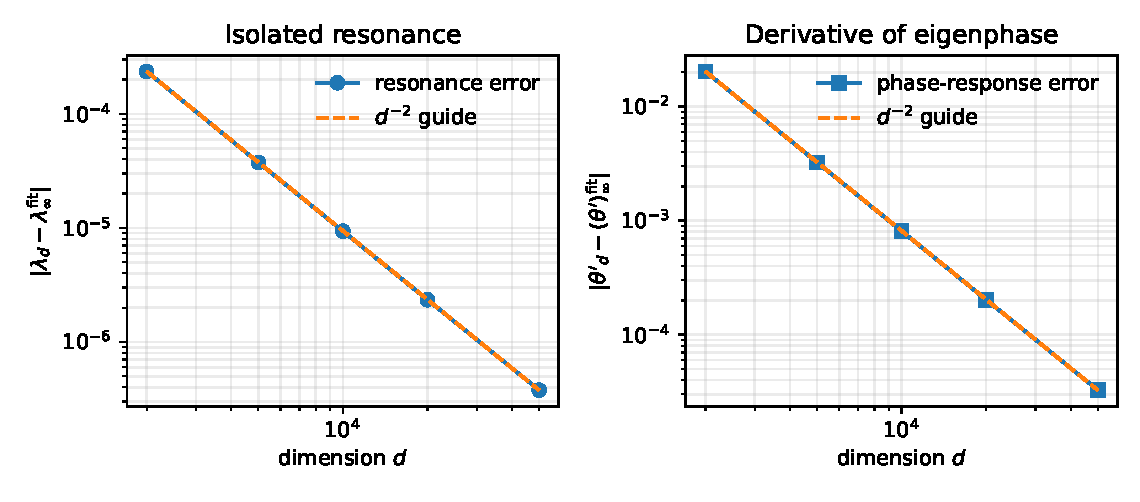
\includegraphics[width=0.78\textwidth]{figures/spectral_extrapolation.pdf}
\caption{Second-order Nystr\"om convergence to the fitted six-sigma continuum
branch.  Both the nonreal resonance and its analytic eigenphase derivative
follow the $d^{-2}$ guide across the full measured range.}
\label{fig:spectral}
\end{figure}

The agreement in \cref{fig:spectral} verifies the rate predicted by
\cref{thm:spectral-convergence} for this isolated branch.  It does not by
itself prove the continuum theorem, and the fitted limit is not an arithmetic
target.

\subsection{Strong versus weak conditional sampling}

To isolate sampling topology, choose a representative Gaussian row at
$u=1.5437$, source position $x=0.8$, and the untuned width $\sigma=0.05$.
For dimensions from $64$ through $2048$, assign
\[
  N_d=\left\lfloor\frac{10^8}{d}\right\rfloor
\]
independent destination samples and repeat the multinomial experiment 500
times.  The weak observable is
\[
  g(y)=\cos(\pi y)+0.3\sin(2\pi y).
\]
The scripts use NumPy for sampling and Matplotlib for the publication figures
\citep{HarrisEtAl2020,Hunter2007}.

The fitted dimension exponents over $d\ge256$ are
\begin{equation}\label{eq:measured-slopes}
  \E\norm{\widehat p-p}_1\asymp d^{1.0046},
  \qquad
  \left(\E|(\widehat p-p)g|^2\right)^{1/2}
  \asymp d^{0.4827},
\end{equation}
at fixed total transition budget.  They agree with the theoretical exponents
$1$ and $1/2$.

\begin{figure}[t]
\centering
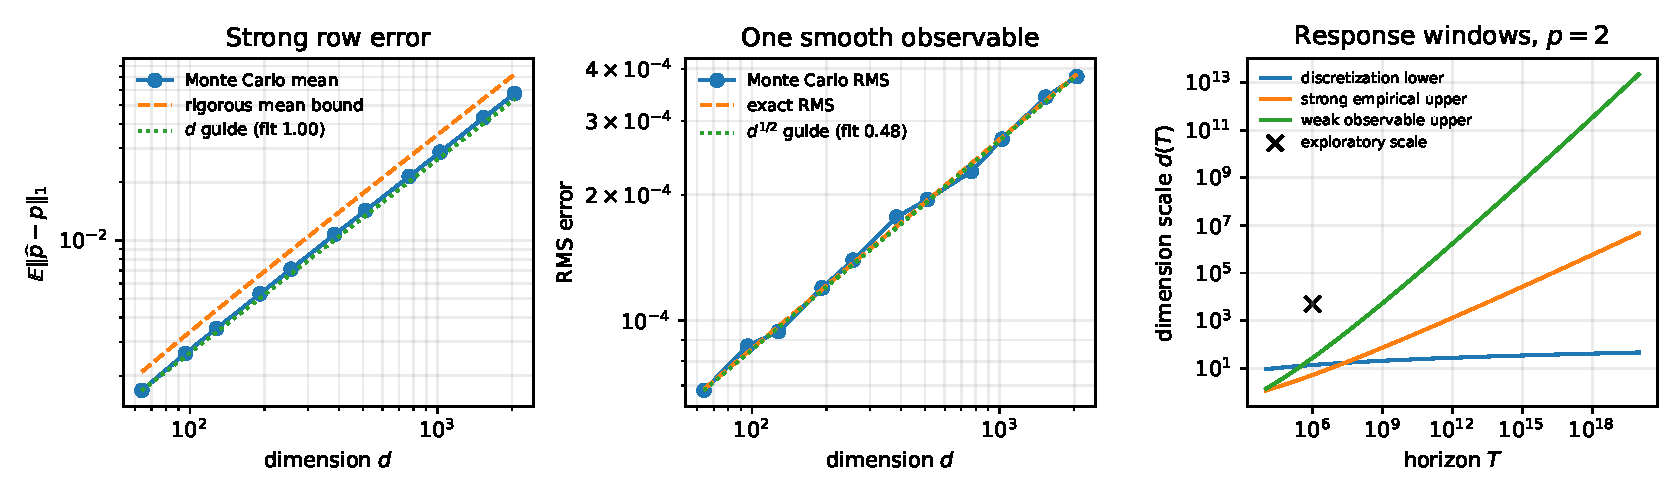
\includegraphics[width=\textwidth]{figures/sampling_windows.pdf}
\caption{Sampling topology and response windows.  Left: complete-row
total-variation error follows $d/\sqrt T$ and stays below the rigorous
multinomial mean bound.  Middle: one smooth observable follows
$\sqrt{d/T}$ and agrees with its exact multinomial RMS.  Right: the
deterministic lower scale and the weak and strong upper scales for $p=2$.
The marked exploratory point used deterministic probability propagation and
therefore is not subject to the empirical upper curves.}
\label{fig:sampling}
\end{figure}

For $p=2$ and $T=10^6$, the unit-constant scales are
\[
  (\log T)^{p/2}=13.82,\qquad
  \frac{\sqrt T}{(\log T)^p}=5.24,\qquad
  \frac{T}{(\log T)^{2p}}=27.45.
\]
Thus there is not yet a unit-constant strong empirical window, while a narrow
weak window is visible.  These values are illustrative, because asymptotic
little-$o$ conditions do not specify universal finite constants.  More
importantly, a deterministic full-cloud computation has no sampling upper
bound at all.  It can still retain an atomic initial-layer bias: at
$d=5000$ and $T=10^6$,
\[
  \frac{d/T}{(\log T)^{-2}}\approx0.95,
\]
so the first unsmoothed source row is not negligible on the nominal response
scale unless it is discarded or separately subtracted.

\section{Implications for quadratic spectral models}
\label{sec:implications}

\subsection{What the continuum theorem supplies}

At fixed physical noise, the finite matrices are not free-standing spectral
lists.  They are Nystr\"om representations of the explicitly defined compact
operator \eqref{eq:continuum-operator}.  Nonzero isolated matrix resonances
converge with multiplicity, and a simple branch has a controlled derivative.
This turns the observed $d^{-2}$ law into a consequence of smooth quadrature
rather than an unexplained numerical pattern.

The theorem also identifies what must be centered.  The unscaled long
exposure freezes to $\cK_{\uc}$; the first logarithmic spectral response is
the derivative \eqref{eq:continuum-response}.  Grid refinement can accompany
this limit only when the deterministic branch bias is $o(s_T)$.

\subsection{Why the estimator must be named}

Three objects that look similar in code have different admissible limits:
\begin{enumerate}[label=(\roman*),leftmargin=2.2em]
  \item an unweighted average of deterministic kernels has only the
  discretization lower bound;
  \item row-normalized expected flow also needs control of any atomic initial
  layer but has no Monte Carlo variance; and
  \item a single-trajectory conditional matrix must resolve both source visits
  and destination distributions.
\end{enumerate}
Calling all three a transition matrix hides the factor $\sqrt d$ separating
weak and strong estimation.

\subsection{What remains open}

The present result fixes $\sigma>0$.  If $\sigma$ shrinks with $h$, the
continuum operator changes toward deterministic composition and the raw
matrix derivative norms can diverge \citep{WangGaussianResponse2026}.  A
triple limit in $T,d,\sigma$ therefore requires a different Banach topology.

Likewise, operator averages forget temporal order.  After continuum and
sampling control, the next order-sensitive object should be a parity-resolved
two-step cocycle or a centered trace response
\citep{WangParity2026}.  Any comparison with arithmetic fluctuations would
then require target-independent parameters, independent unfolding, and a
separate theorem.  None is asserted here.

\section{Conclusion}

The fixed-noise Gaussian quadratic model has a rigorous continuum spectral
meaning.  Its normalized kernel is a compact, strongly positive analytic
Markov operator, and midpoint Nystr\"om matrices are collectively compact
spectral approximations.  Every nonzero isolated resonance is free of
nonzero spectral pollution; simple resonance and eigenphase responses converge
at second order.

The joint time--resolution problem is not described by one universal window.
Deterministic probability propagation needs only to make the $d^{-2}$ bias
smaller than the logarithmic response.  A weak observable estimated from
conditional samples costs $\sqrt{d/T}$, while a complete row in total
variation costs $d/\sqrt T$.  Strong matrix control is consequently much more
restrictive than a successful observable plot, exactly as the multinomial
experiments demonstrate.

These results complete the continuum and sampling foundation for the
renormalized Gaussian response.  They do not convert Markov resonances into
self-adjoint energies, identify them with Riemann zeros, or imply the Riemann
hypothesis.

\section*{Data and code availability}

The manuscript source, tests, machine-readable results, and figure scripts
are available at
\url{https://github.com/maris205/prime_dynamics_theory/tree/main/papers/continuum-spectral-double-limits}.
The spectral extrapolation reads the published benchmark data from the
preceding paper in the same repository.

\section*{Acknowledgments}

The author acknowledges the use of an AI language model for assistance with
mathematical cross-checking, code development, manuscript organization, and
typesetting.  The author verified the final arguments and assumes
responsibility for the content.

{\small
\bibliographystyle{plainnat}
\bibliography{references}
}

\end{document}
